\chapter{Theorie}
\section{Grundlagen MRT}
Die Magnetresonanztomographie (MRT) ist ein Bildgebendes Verfahren, bei der keine ionisierende Strahlung eingesetzt wird.
Dadurch gibt es keine Strahlenbelastung für Patientinnen und Patienten.
Die MRT wird zur Darstellung von morphologischen Strukturen und zur Abbildung funktioneller Prozesse verwendet.
Das MRT-Gerät besteht aus einem zylinderförmigen, supraleitenden Magneten, der ein homogenes Hauptmagnetfeld $B_0$ erzeugt. %Shimming optional
In der klinischen Anwendung liegt die Magnetfeldstärke bei $\qty{1.5}{T}$ - $\qty{3}{T}$.~\cite{Schlegel}
Die Kernteilchen besitzen ein magnetisches Moment $\vec{m}$, aufgrund dessen das sie um die Achse des Magnetfeldes $B_0$, mit der Lamorfrequenz 
\begin{equation}
    \omega_0 = \gamma \cdot B_0
\end{equation}
präzedieren. Dabei beschreibt $\gamma$ das Gyromagnetische Verhältnis, welches Materialabhängig ist.
Befinden sich diese Atome im Magnetfeld,
richten sich die Spins der Kernteilchen parallel und antiparallel nach dem Magnetfeld aus. Sie befinden sich im thermischen Gleichgewicht.
Bei Atomen mit einer geraden Anzahl an Kernteilchen heben sich beim aufsummieren die magnetischen Momente auf und besitzen somit keine
Magnetisierung. 
Da die Magnetisierung notwendig für die Messung eines Signals im MRT ist, können nur Atome mit einer ungeraden Anzahl an Kernteilchen gemessen werden.
Am häufigsten wird zur Messung Wasserstoff verwendet, da dies mit ca. $\qty{80}{\%}$ am häufigsten im Menschlichen Körper vorkommt.
Mittels eines Hochfrequenzsignals (HF) werden die Spins um einen Winkel
\begin{equation}
    \alpha = \gamma \cdot B_1 \cdot T 
\end{equation}
gekippt. Dabei entspricht $B_1$ dem Anregungsimpuls und $T$ die Zeit des HF-Impulses.
Die Frequenz des HF-Signals entspricht der Lamorfrequenz des Kernspins, damit es zur Resonanz kommt. 
Beim Ausschalten des Signals, relaxieren die Spins zurück in ihre Gleichgewichtsmagnetisierung. 
Dabei wird zwischen T1-Relaxation und T2-Relaxation unterschieden. 
%Mittels dieser Unterscheidung und der Einstellung der Echozeit $T_E$ und 
%Repetitionszeit $T_R$, sind die Bilder unterschiedlich Gewichtet.
Die Repetitionszeit $T_R$ beschreibt die Zeit zwischen der Verwendung zweier HF-Impulse und die Echozeit $T_E$ der zeitliche Abstand zwischen dem Anregungsimpuls und der Auslesung des Signals. 
Anhand der Gewichtungen entstehen unterschiedliche Kontraste.
Durch die veränderten Magnetisierung kommt es zur Induktion einer Spannung, die mittels einer Spule gemessen wird.~\cite{Pollmann}

Bei der T1- Relaxation wird die Längsmagnetisierung betrachtet, welche mit der Zeit zunimmt.
Diese lässt sich durch 
\begin{equation}
    M_z(t) = M_z(0) (1 - e^{-\frac{t}{T_1}})
\end{equation}
Der Zeitpunkt $T_1$ wird nach der Anregung bestimmt, bei dem $\qty{63}{\%}$ der Magnetisierung wiederhergestellt wurde.~\cite{Pollmann}\\
%Bei der T1 Gewichtung, sind $T_R$ und $T_E$ kurz eingestellt und zusätzlich gilt das $T_E \ll T_2$.
%Fett und Muskeln werden bei dieser Gewichtung hell dargestellt und Liquor dunkel.~\cite{Schlegel}
Die T2-Relaxation beschreibt die Quermagnetisierung, welche mit der Zeit abnimmt, da die Spins dephasieren und somit das Signal zerfällt.~\cite{Dössel}
Die Magnetisierung wird durch die Formel
\begin{equation}
    M_{xy}(t) = M_{xy}(0) e^{-\frac{t}{T_2}} 
\end{equation}
beschrieben.
Wenn die transversale Magnetisierung auf $\qty{37}{\%}$ abgefallen ist, wird der zeitpunkt $T_2$ bestimmt.~\cite{Pollmann}
%Für T2-Gewichtete Bilder gilt, dass $T_R \gg T_1$ und sowohl $T_R$ als auch $T_E$  lang eingestellt werden. 
%Bei dieser Gewichtung wird Liquor hell dargestellt und Fett und Muskeln dunkel.~\cite{Schlegel} 
Aufgrund von Inhomogenitäten im Hauptmagnetfeld, kommt es zu einem schnelleren Signalzerfall. Dies wird bezeichnet als T2* Relaxation.
Dieser Signalzerfall wird als "Free Induction Decay" (FID) bezeichnet.~\cite{Dössel}\\

Für die Erstellung des Bildes, benötigt es die drei Gradientenspulen $G_z$, $G_y$ und $G_x$. Die Anordnung der drei Spulen 
ist in Abbildung \ref{fig:an Grad} abgebildet.
\begin{figure}[H]
  \centering
  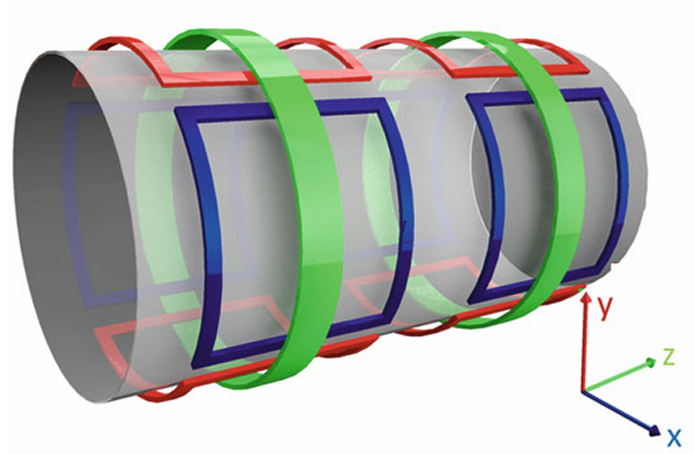
\includegraphics[scale=0.4]{/nfs/homes/sdreyer/Digit-Classification-Pytorch/tudothesis-main/content/abbildungen/Anordnung Gradientenspulen.png}
  \caption{Anordnung der Gradientenspulen.\cite{Schlegel}}
  \label{fig:an Grad}
\end{figure}
Durch das schalten der Gradienten kommt es zur Überlagerung mit dem Magnetfeld, wodurch die Codierung des Bildes möglich ist.
Der Gradient in z-Richtung wird für die Einstellung der Schichtdicke verwendet. 
Zur Frequenzcodierung wird der Gradient $G_x$ geschaltet, wodurch sich die Lamorfrequenzen entlang des Gradienten verschieben.
Mittels des Gradienten $G_y$ werden die Spins in ihrer Phase verschoben.
Durch die Verschiebung der Frequenz und Phase ist die Ortscodierung möglich und die Aufnahme eines Bildes im k-Raum.
Durch die Fouriertransformation werden die Informationen in den Ortsraum transformiert.
Dadurch liefert die MRT Bilder in Schichten, die anschließend zu einem 3D-Bild zusammengesetzt und analysiert werden.~\cite{pabst2013}

\section{Maschinelles Lernen}
Künstliche Intelligenz (KI) bezeichnet die Modellierung menschlicher Intelligenz durch Maschinen. 
Das Maschinelle Lernen (ML) ist ein Teilbereich der Künstlichen Intelligenz. Deep Learning stellt 
wiederum einen Teilbereich des maschinellen Lernens da. Das Deep learning beinhaltet das trainieren mehrschichtiger Neuronaler Netzwerke mit großen Datensätzen.
Die verschieden Teilbereiche der Künstliche Intelligenz werden in der Abbildung \ref{fig:KI} dargestellt.
Durch die Verwendung von Daten ist es den Algorithmen beim 
Maschinellem Lernen möglich aus diesen zu lernen und sich zu verbessern, ohne das die Algorithmen dem Problem entsprechend programmiert werden müssen.~\cite{kleesiek2020}
Somit findet das Maschinelle Lernen Anwendung in der Identifizierung und Klassifikation von Objekten, Analyse, Vorhersagen, 
Sprachverarbeitung, Informationsbeschaffung und in weiteren Bereiche.~\cite{shinde2018}
\begin{figure}[H]
  \centering
  \includegraphics[scale=0.4]{/nfs/homes/sdreyer/Digit-Classification-Pytorch/tudothesis-main/content/abbildungen/Künstliche Intelligenzpng.png}
  \caption{Künstliche Intelligenz und ihre Teilbereiche.~\cite{kleesiek2020}}
  \label{fig:KI}
\end{figure}
Das Lernen lässt sich unterscheiden in überwachtes Lernen (Supervised Learning) und unüberwachtes Lernen (Unsupervised Learning).
Beim überwachten Lernen, sind die Eingabedaten gelabelt, sodass das Netzwerk anhand dessen lernt, indem es den Ausgabewert mit dem bekannten Zielwert 
vergleicht und das Netzwerk dementsprechend anpasst.
Beim unüberwachten Lernen erkennt der Algorithmus Muster und Strukturen in den Eingabedaten, ohne das Eingabedaten gelabelt sind.~\cite{kleesiek2020}
\subsection{Neuronales Netzwerk}
Das Neurale Netzwerk ist aufgebaut aus drei Schichten: 
Die Eingabeschicht (Input Layer), versteckten Schichten (Hidden Layers) und die Ausgabe Schicht (Output Layer).
Die Input Layer nimmt die Daten auf und den Neuronen wird ein Wert zugeordnet.
Bei den Hidden Layers handelt es sich um mehrere Schichten, die sich zwischen der Eingabe- und Ausgabeschicht befinden.
In diesen werden die Eingabedaten verarbeitet und die Ergebnisse an die Ausgabeschicht weitergegeben.
Die Neuronen der versteckten Schichten erhalten dabei keine Daten von Außerhalb und geben keine raus. 
Der Aufbau eines Neuronalen Netzwerkes wird in der Abbildung \ref{fig:NN} dargestellt.
\begin{figure}[H]
  \centering
  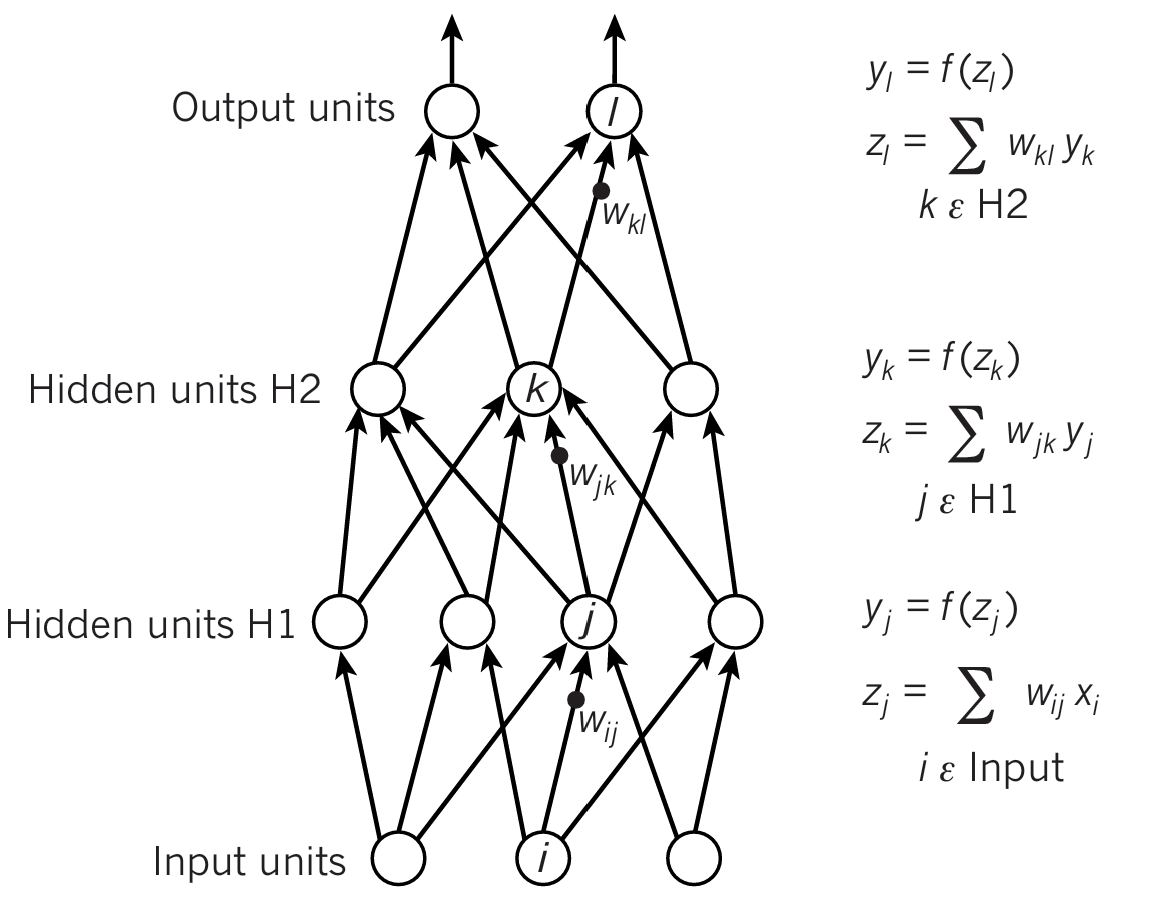
\includegraphics[scale=0.4]{/nfs/homes/sdreyer/Digit-Classification-Pytorch/tudothesis-main/content/abbildungen/Aufbau NN.png}
  \caption{Aufbau eines Fully Connected Neural Network.~\cite{lecun2015deep}}
  \label{fig:NN}
\end{figure}
Die nachfolgende Beschreibung bezieht sich auf den Aufbau dieses Netzwerkes.
Jedes Neuron ist dabei mit jedem aus der Vorherigen Schicht verbunden durch eine Gewichtung $w_{ij}$.
Die Aktivierung eines Neurons wird mittels einer Aktivierungsfunktion $f_\text{act}$ berechnet. In dieser fließt unter anderem die Gewichtung, 
der Eingabe Wert $x_i$ sowie ein Bias-Wert $b_j$ mit ein.
Der Output des Neurons j lässt sich somit über 
\begin{equation}
    y_j = f_\text{act}\left(\sum_{i}^{n} w_{ij}x_i + b_j\right)
\end{equation}
berechnen.
Dieser Ausgabewert $y_j$ wird an die Neuronen in der nächsten Schicht weitergegeben.
Die meist verwendetet Aktivierungsfunktionen sind die Sigmoidfunktion, Rectifier-Funktion (ReLU-Funktion) und der hyperbolische Tangens.
Wird der Schwellenwert bei diesen Funktionen nicht erreicht, wird der Wert des Neurons nicht an die nächste Schicht weitergegeben.
Das Neuron wird inaktiv.
Bei der ReLU-Funktion beträgt der Schwellenwert 0, sodass die Ausgangswerte nur im positiven Bereich liegen.
Die Sigmoidfunktion gibt einen Ausgabewert zwischen 0 und 1, da diese Funktion auf diesen Wertebereich normalisiert ist.
Beim verwenden des hyperbolischen Tangens, befindet sich der Wertebereich zwischen -1 und +1.~\cite{datascience}

\subsection{Convolutional Neural Network}\label{sec:NN}
Für die Verarbeitung von Bildern eignet sich das Fully Connected Neural Network, wie es in \ref{fig:NN} dargestellt ist, nicht, da jedes Pixel ein Eingabewert darstellt.
Aufgrund der Verbindung jedes Neurons aus der vorherigen Schicht, kommt es zu einer großen Anzahl an Verbindungen.
Durch die große Anzahl an Rechenoperationen ist das Training des Netzwerkes ineffizient.
Aus diesem Grund und zur Nutzung der räumlichen Korrelation der Pixel wird für die Verarbeitung von Bildern das Convolutional Neural Network (CNN) verwendet.
Bei diesem sind die Neuronen in drei Dimensionen angeordnet.
Diese sind die zwei räumlichen Dimensionen Breite und Höhe und die dritte Dimension bildet die Anzahl an Kanälen.
Der Beispielhafte Aufbau eines CNN in seiner Standardform wird in der Abbildung \ref{fig:CNN} dargestellt.
Dabei ist das Netzwerk aufgebaut aus Faltungschichten (Convolutional Layers), Pooling Layers und einer Fully-Connected Layer (FC-Layer).
Zwischen den Schichten wird, wie bei den Neuronalen Netzwerken eine Aktivierungfunktion verwendet.~\cite{OShea} 
\begin{figure}[H]
  \centering
  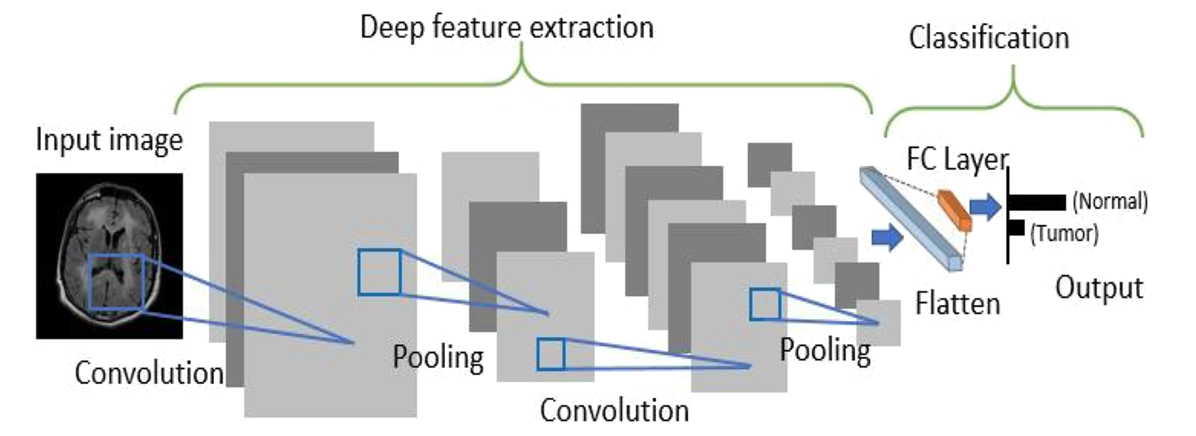
\includegraphics[scale=0.3]{/nfs/homes/sdreyer/Digit-Classification-Pytorch/tudothesis-main/content/abbildungen/CNN.png}
  \caption{Aufbau eines Convolutional Neural Network.~\cite{Mohammed2024}}
  \label{fig:CNN}
\end{figure}
Bei der Convolutional Layer, wird ein Filter (Kernel) verwendet, welcher schrittweise über das gesamte Input Bild gelegt wird.
Dieser besitzt meist eine typische Größe von $3 \times 3$, $5 \times 5$ oder $ 7 \times 7$.  
Aus dem Kernel und dem Neuron wird das Skalarprodukt berechnet, aus dem eine Feature-Map erstellt wird. 
Diese Feature-Map beinhaltet die wichtigsten Strukturen und Merkmale.~\cite{Yamashita2018}
Der Ausgabewert der Feature-Map an der Position (i,j) ergibt sich durch die Faltung
\begin{equation}
  S(i,j) = (K * I)(i, j) = \sum_m \sum_n I(i + m, j + n) \cdot K(m,n).
\end{equation}
Dabei beschreibt $I$ das Eingabebild und $K$ den Kernel.~\cite{Goodfellow-et-al-2016}
Damit der Filter auch den Rand des Bildes mit dem Zentrum überlappen kann, wird das sogenannte Padding angewendet.
Beim Zero-padding, werden am Rand des Bildes Nullen hinzugefügt. Dadurch bleibt die räumliche Dimension erhalten.
Als Stride wird der Abstand zwischen zwei Positionen des Kernels beschrieben. Am häufigsten wird ein stride von 1 gewählt. 
Das bedeutet, dass sich nach jeder Berechnung des Skalarproduktes der Kernel um eine Position verschiebt.
\begin{figure}[H]
  \centering
  \begin{subfigure}[b]{0.3\textwidth}
    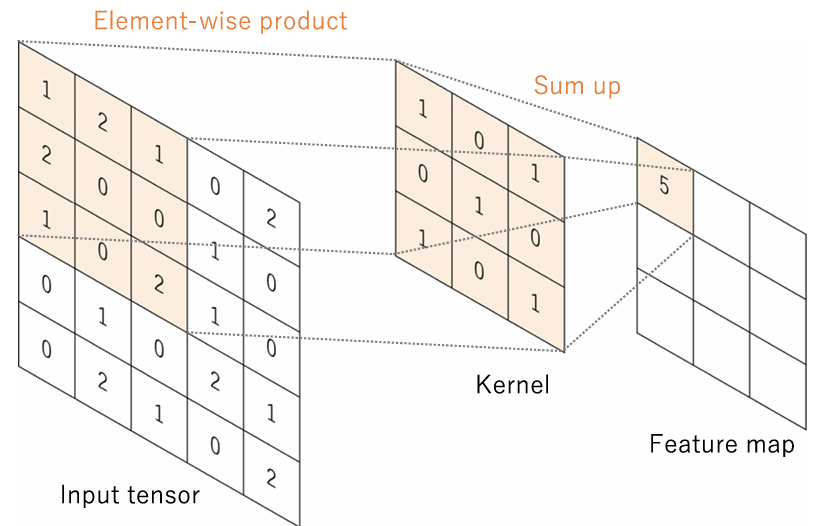
\includegraphics[width=\textwidth]{/nfs/homes/sdreyer/Digit-Classification-Pytorch/tudothesis-main/content/abbildungen/kernel a.png}
    %\caption{}
    \label{}
  \end{subfigure}
  \hfill
  \begin{subfigure}[b]{0.3\textwidth}
    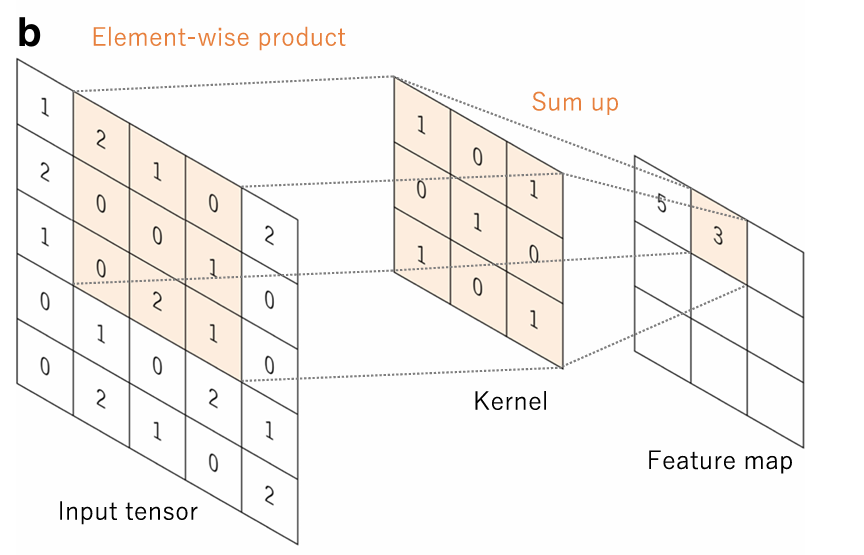
\includegraphics[width=\textwidth]{/nfs/homes/sdreyer/Digit-Classification-Pytorch/tudothesis-main/content/abbildungen/kernel b.png}
    %\caption{}
    \label{}
  \end{subfigure}
  \hfill
  \begin{subfigure}[b]{0.3\textwidth}
    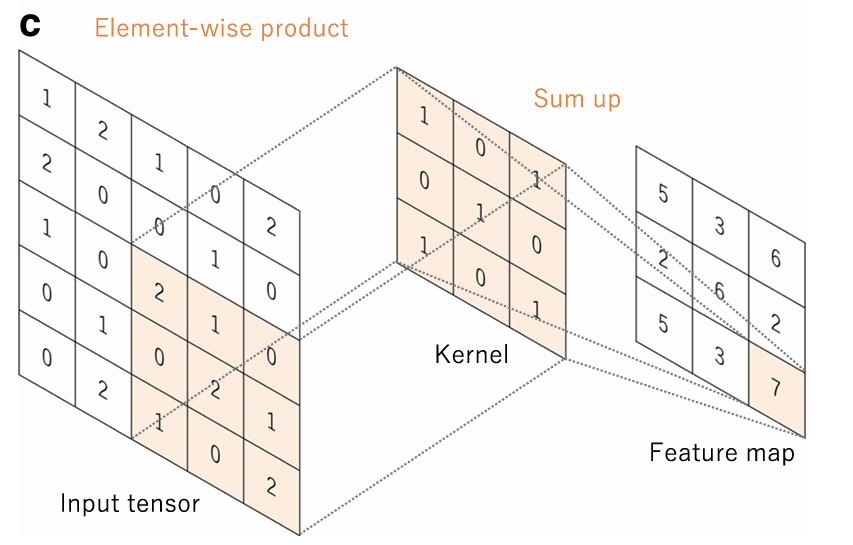
\includegraphics[width=\textwidth]{/nfs/homes/sdreyer/Digit-Classification-Pytorch/tudothesis-main/content/abbildungen/kernel c.png}
    %\caption{}
    \label{}
  \end{subfigure}
  \caption{Ein Beispiel der Convolutional layer mit der Verwendung eines Kernels der Größe $3 \times 3$.~\cite{Yamashita2018}}
  \label{fig:kernel}
\end{figure}
Die Pooling-Layer reduziert die räumliche Dimension. Infolge dessen kommt es auch zur Reduktion der Parameter.~\cite{datascience}
Dafür wird das sogenannte Max-Pooling verwendet. Dabei wird ein Filter der Größe $2 \times 2$ verwendet, der wie der Kernel, schrittweise über die Feature-Map gelegt wird.
Für jeden Ausschnitt wird der größte Wert verwendet. Der Rest der Werte wird nicht weiter verwendet.~\cite{Yamashita2018}\\
%Dies wird in der Abbildung 
%\begin{figure}[H]
%  \centering
%  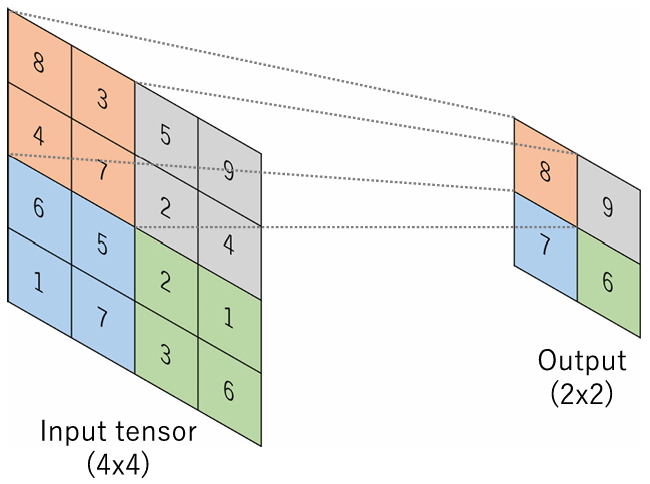
\includegraphics[scale=0.4]{/nfs/homes/sdreyer/Digit-Classification-Pytorch/tudothesis-main/content/abbildungen/max_pooling.png}
%  \caption{Eine Beispielhafte Anwendung von Max-Pooling mit einem $2 \times 2$ Filter.~\cite{Yamashita2018}}
%  \label{fig:CNN}
%\end{figure}
Die FC-Layer berechnet am Ende die Aktivierung und bestimmt einen Ausgangswert für die Klassifizierung.
Sie entspricht damit der Art von Output-Layer, die in Kapitel \ref{sec:NN} beschrieben wurde.

\subsection{Training eines Netzwerkes}
Beim Training der Netzwerke, werden die Gewichtungen zwischen den Neuronen schrittweise angepasst. 
Zu Beginn wird den Gewichtungen ein Zufälliger Wert zu geschrieben.
Beim Training, wird zur Anpassung der Gewichtungen der Backpropagation-Algorithmus verwendet.
Dabei wird die sogenannte Verlustfunktion (Loss Function) angewendet, welche den Fehler zwischen dem Ausgabewert des Netzwerkes und den bekannten Zielwert berechnet.
Ziel des Training ist es das Minimum der Verlustfunktion zu ermitteln, indem die Parameter angepasst werden.~\cite{datascience}
Häufige Verlustfunktionen sind beispielsweise der Mean Squared Error (MSE)
\begin{equation}
  \text{MSE}  =  \frac{1}{n} \sum_{i=1}^{n} (y_i - \hat{y}_i)^2
\end{equation}
oder die Binary Cross-Entropie für die Klassifikation zwischen zwei Klassen  
\begin{equation}
\text{CE} = -\frac{1}{n} \sum_{i=1}^{n} \left( y_i \cdot \log(\hat{y}_i) + (1 - y_i) \cdot \log(1 - \hat{y}_i) \right).
\label{eq:BCE}
\end{equation}
Dabei beschreibt $n$ die Anzahl an Training samples, $y_i$ den Zielwert und $\hat{y}_i$ den berechneten Ausgabewert.
Durch den Backpropagation-Algorithmus wird die partielle Ableitung der Verlustfunktion mittels der Kettenregel berechnet.
Da der Gradient in die Richtung des größten Anstiegs zeigt, erfolgt die Anpassung der Gewichte in die entgegengesetzte Richtung. 
Eine positive Ableitung führt somit zur Verringerung, eine negative zur Erhöhung der Gewichtung.~\cite{neuralnet}
Der Optimizer passt auf Grundlage des Gradienten die Parameter an und sorgt dafür, dass diese im Netzwerk aktualisiert werden.
Zu den häufigsten verwendeten Optimizer sind der SGD, RMSprop und Adam.
Zusätzlich wird beim Training eine Validierung durchgeführt um die Hyperparameter zu optimieren. 
Hierzu wird der Datensatz aufgeteilt, in Training- und Validierungsdaten, wobei die Validierungsdaten nicht zur Aktualisierung 
der Gewichtungen verwendet werden.~\cite{Yamashita2018}
Als Hyperparameter werden die Parameter bezeichnet, die zu Beginn des Trainings manuell festgelegt werden.
Zu diesen gehört unter anderem die Lernrate, die Batch-Größe, die Anzahl an Schichten und Neuronen, die Anzahl an Trainingsdurchläufen (Epochen)
und die Verlustfunktion.
Die Batch-Größe gibt an, wie viele Trainingsdaten pro Trainingsschritt verwendet werden.~\cite{datascience} 
Die Lernrate legt fest, wie stark die Gewichte bei jedem Trainingsschritt angepasst werden.~\cite{Mohammed2024} 
Um Overfitting zu vermeiden, wird der sogenannte Dropout als weiterer Hyperparameter eingebaut.
Der Dropout schaltet während des Trainings zufällige Neuronen aus.
Dadurch stützt sich das Netzwerk nicht auf Spezifische Neuronen und das Netzwerk wird robuster. ~\cite{Yamashita2018}.

Wenn ein Modell neben den relevanten Mustern auch die irrelevante Störungen lernt, die nur in den Trainingsdaten enthalten sind, gilt es als zu stark an den Trainingsdaten angepasst.
Bei der Anwendung des Netzwerkes auf einen unabhängigen Datensatz, verschlechtert sich die Leistung deutlich. 
Dieses Verhalten wird dann als Overfitting bezeichnet.
Um zu überprüfen, ob das Modell überangepasst ist, wird der Validierungsverlust (Validation Loss) während des Trainings mitbeobachtet.
Wenn der validation loss ansteigt, der Trainings Verlust jedoch kontinuierlich sinkt, ist dies ein Zeichen, dass das Netzwerk überangepasst wird.~\cite{Yamashita2018}
Dies wird in der Abbildung \ref{fig:overfitting} graphisch dargestellt.
\begin{figure}[H]
  \centering
  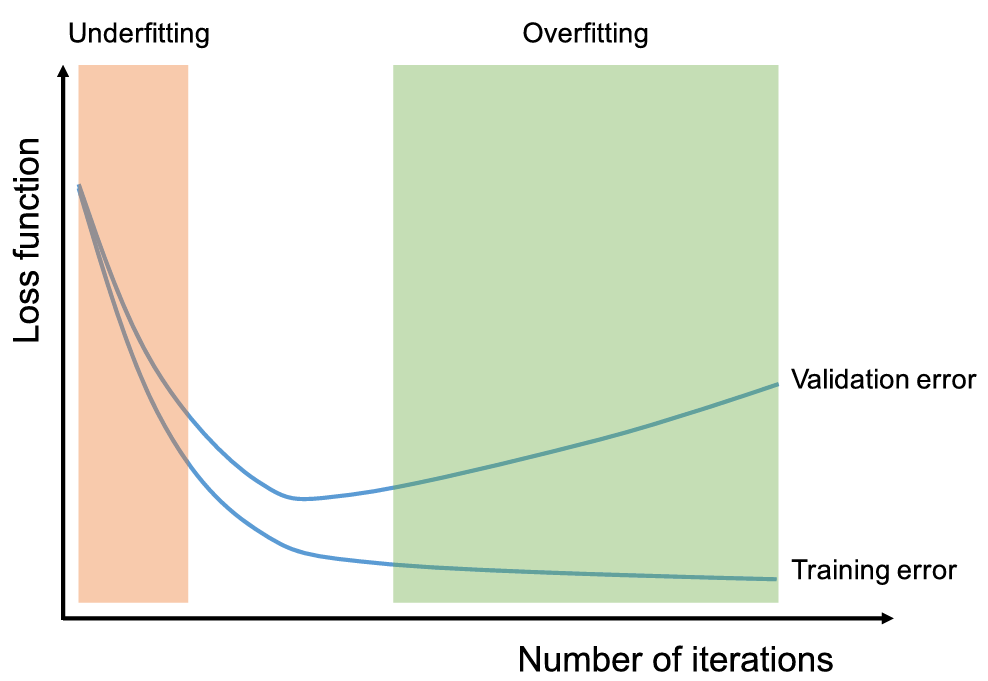
\includegraphics[scale=0.23]{/nfs/homes/sdreyer/Digit-Classification-Pytorch/tudothesis-main/content/abbildungen/Overfitting.png}
  \caption{Überprüfung auf Overfitting durch das Kontrollieren des Trainings und validation loss.~\cite{Yamashita2018}}
  \label{fig:overfitting}
\end{figure}
%Möglichkeiten um Overfitting zu vermeiden sind zum einen, das mehr Daten verwendet werden. 
%Zudem kann ein Dropout implementiert werden. Der Dropout schaltet während des Trainings zufällige Neuronen aus.
%Dadurch stützt sich das Netzwerk nicht auf Spezifische Neuronen 